% 保留原始面板、实拍、示例与全部连线；仅以 TikZ 覆盖说明标签。
\begin{tikzpicture}
\node[anchor=south west,inner sep=0] (im) at (0,0) {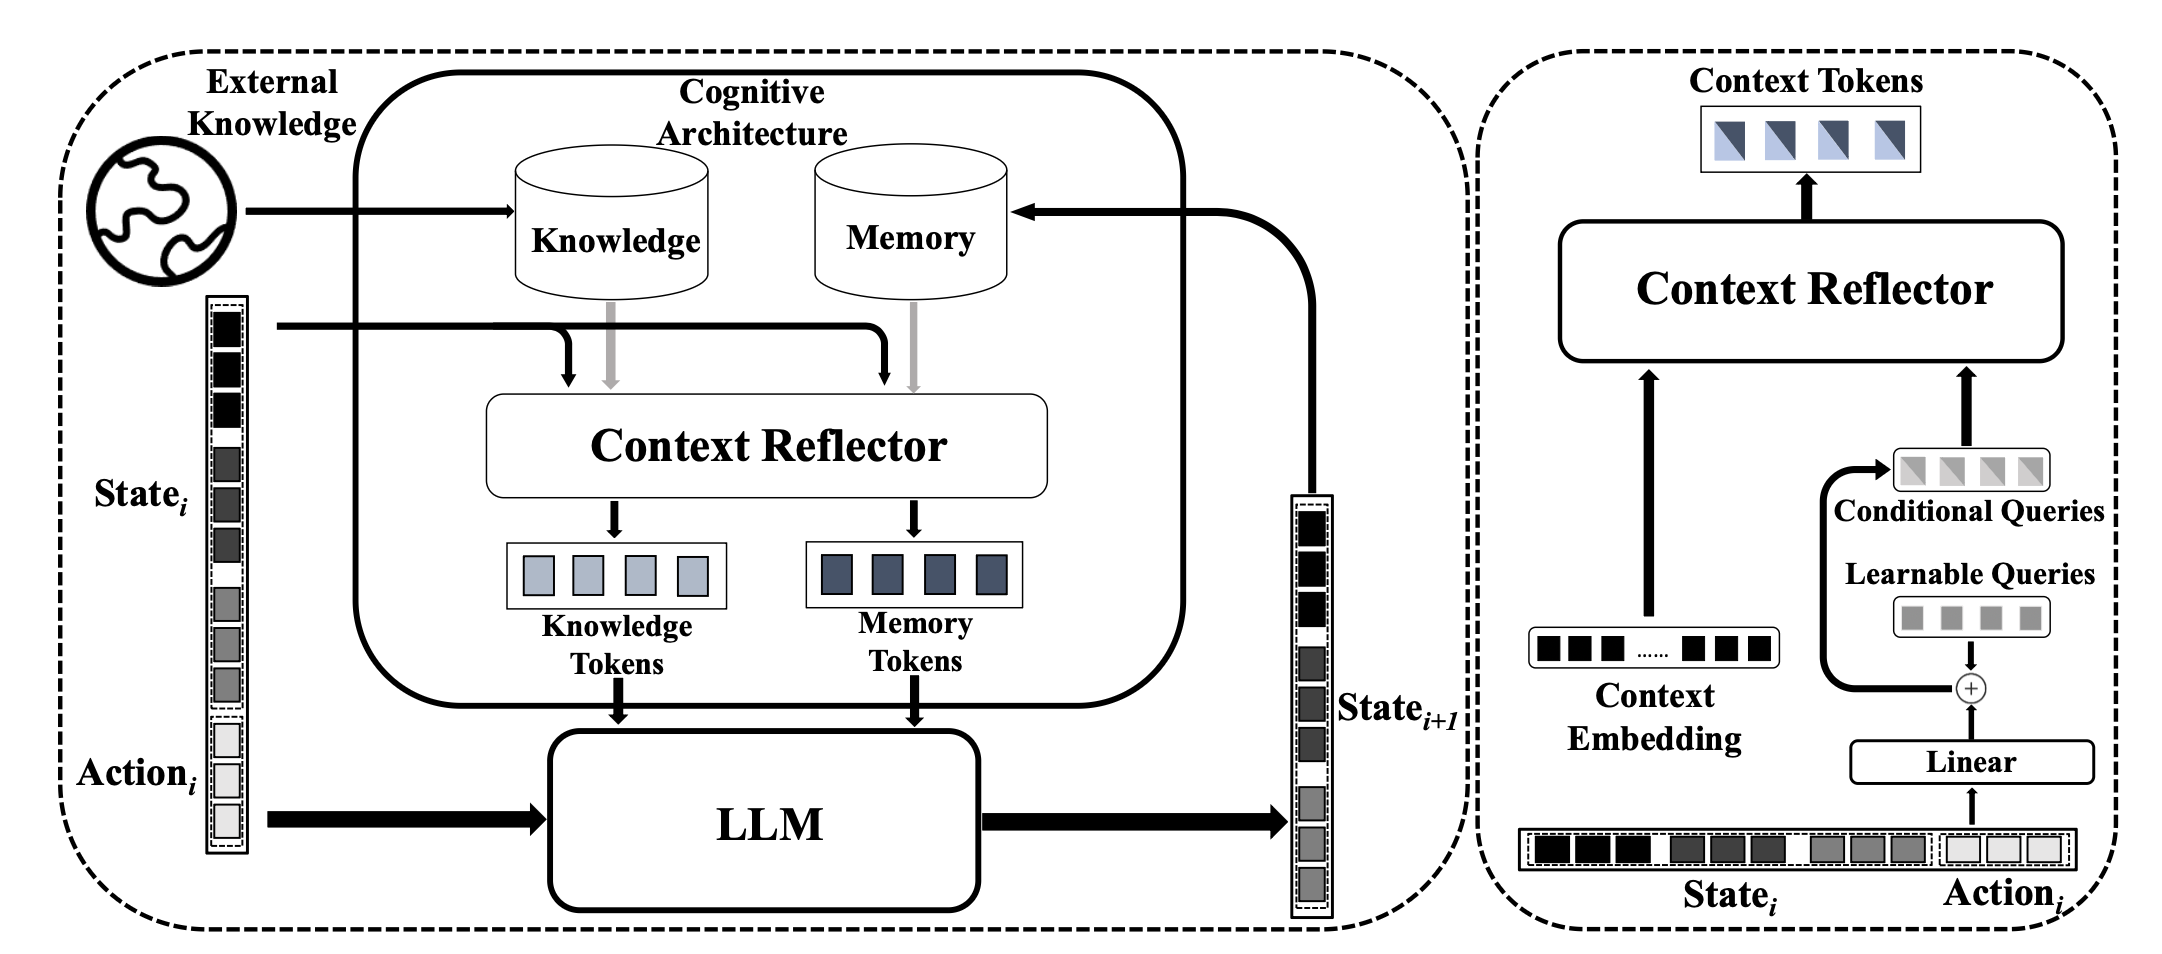
\includegraphics[width=\linewidth]{figures/worldgpt.png}};
\begin{scope}[x={(im.south east)},y={(im.north west)}]
\fill[white] (0.082500,0.850000) rectangle (0.167500,0.940000);
\node[align=center,inner sep=0pt,font=\fontsize{8.5}{9.5}\selectfont,text width=0.085000\linewidth,rotate=0] at (0.125000,0.895000) {外部\\知识};
\fill[white] (0.300293,0.838496) rectangle (0.411133,0.921460);
\node[align=center,inner sep=0pt,font=\fontsize{8.5}{9.5}\selectfont,text width=0.110840\linewidth,rotate=0] at (0.355713,0.879978) {认知架构};
\fill[white] (0.239000,0.723500) rectangle (0.329000,0.778500);
\node[align=center,inner sep=0pt,font=\fontsize{9}{10}\selectfont,text width=0.090000\linewidth,rotate=0] at (0.284000,0.751000) {知识};
\fill[white] (0.386000,0.725500) rectangle (0.466000,0.780500);
\node[align=center,inner sep=0pt,font=\fontsize{9}{10}\selectfont,text width=0.080000\linewidth,rotate=0] at (0.426000,0.753000) {记忆};
\fill[white] (0.242000,0.498000) rectangle (0.472000,0.566000);
\node[align=center,inner sep=0pt,font=\fontsize{10}{11}\selectfont,text width=0.230000\linewidth,rotate=0] at (0.357000,0.532000) {上下文反思器};
\fill[white] (0.238500,0.278000) rectangle (0.333500,0.366000);
\node[align=center,inner sep=0pt,font=\fontsize{8.5}{9.5}\selectfont,text width=0.095000\linewidth,rotate=0] at (0.286000,0.322000) {知识\\词元};
\fill[white] (0.380000,0.280000) rectangle (0.470000,0.368000);
\node[align=center,inner sep=0pt,font=\fontsize{8.5}{9.5}\selectfont,text width=0.090000\linewidth,rotate=0] at (0.425000,0.324000) {记忆\\词元};
\fill[white] (0.029000,0.454000) rectangle (0.099000,0.504000);
\node[align=center,inner sep=0pt,font=\fontsize{8}{9}\selectfont,text width=0.070000\linewidth,rotate=0] at (0.064000,0.479000) {状态$_i$};
\fill[white] (0.021500,0.158000) rectangle (0.096500,0.218000);
\node[align=center,inner sep=0pt,font=\fontsize{8}{9}\selectfont,text width=0.075000\linewidth,rotate=0] at (0.059000,0.188000) {动作$_i$};
\fill[white] (0.614000,0.232500) rectangle (0.678000,0.277500);
\node[align=center,inner sep=0pt,font=\fontsize{7.5}{8.5}\selectfont,text width=0.064000\linewidth,rotate=0] at (0.646000,0.255000) {状态$_{i+1}$};
\fill[white] (0.755000,0.889000) rectangle (0.913000,0.939000);
\node[align=center,inner sep=0pt,font=\fontsize{9}{10}\selectfont,text width=0.158000\linewidth,rotate=0] at (0.834000,0.914000) {上下文词元};
\fill[white] (0.743000,0.657500) rectangle (0.933000,0.722500);
\node[align=center,inner sep=0pt,font=\fontsize{10}{11}\selectfont,text width=0.190000\linewidth,rotate=0] at (0.838000,0.690000) {上下文反思器};
\fill[white] (0.845000,0.440000) rectangle (0.975000,0.480000);
\node[align=center,inner sep=0pt,font=\fontsize{8}{9}\selectfont,text width=0.130000\linewidth,rotate=0] at (0.910000,0.460000) {条件查询};
\fill[white] (0.844000,0.374000) rectangle (0.974000,0.414000);
\node[align=center,inner sep=0pt,font=\fontsize{8}{9}\selectfont,text width=0.130000\linewidth,rotate=0] at (0.909000,0.394000) {可学习查询};
\fill[white] (0.721500,0.191500) rectangle (0.826500,0.276500);
\node[align=center,inner sep=0pt,font=\fontsize{8.5}{9.5}\selectfont,text width=0.105000\linewidth,rotate=0] at (0.774000,0.234000) {上下文\\嵌入};
\fill[white] (0.871000,0.181500) rectangle (0.951000,0.214500);
\node[align=center,inner sep=0pt,font=\fontsize{8}{9}\selectfont,text width=0.080000\linewidth,rotate=0] at (0.911000,0.198000) {线性层};
\fill[white] (0.763500,0.039000) rectangle (0.838500,0.079000);
\node[align=center,inner sep=0pt,font=\fontsize{8}{9}\selectfont,text width=0.075000\linewidth,rotate=0] at (0.801000,0.059000) {状态$_i$};
\fill[white] (0.884766,0.026549) rectangle (0.989258,0.084071);
\node[align=center,inner sep=0pt,font=\fontsize{8}{9}\selectfont,text width=0.104492\linewidth,rotate=0] at (0.937012,0.055310) {动作$_i$};
\end{scope}
\end{tikzpicture}
